\chapter{Existing Similar Games}
\label{competitive-games}

This chapter aims to compare the analyzed game, as described in chapter~\ref{analysis}, with existing similar educational or programming games.
Games will be compared based on criteria found in the conducted survey and studies mentioned in the introduction.
Listed games are selected subjectively as the most related and known by the author.

The conducted survey done in chapter~\ref{survey} found that children players are competitive, they like receiving rewards and ratings and play mostly building games.
Also, in the article~\cite{nand_2019_engaging} they found that challenges were the most appealing, together with feedback~-- with the meaning that players know were scored~-- and graphics.
In the article~\cite{smiderle_2020_the}, similar results were shown while investigating the influence of points, badges, and ranking; as the article states, \textquote{Gamified group participants had a significant improvement in the quality of the submitted solutions, having obtained more accuracy.}
Therefore, this chapter will compare similar games' comprehensibility, story, study materials, graphics, and feedback.
Moreover, because the game \emph{\myAppName} aims at young people, it will also compare their prices.

\newpage
\section{Scratch}
\label{similar-games:scratch}

\begin{figure}
    \centering
    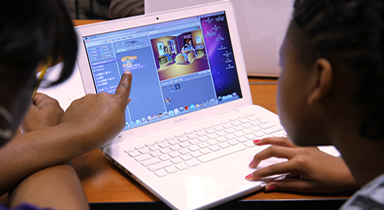
\includegraphics[width=1\linewidth]{assets/similar-games/scratch.jpg}
    \caption{Scratch~\cite{a2022_scratch}}
    \label{fig:scratch}
\end{figure}

Scratch is one of the most extensive coding applications with a simple visual interface that allows the creation of universal programs, as can be seen in figure~\ref{fig:scratch}.
The app presents the user with a large set of code commands, sounds, and an editor of characters.
There are also a few but relatively small sets of tutorials.

Players can create games, animation, and other visual creations.
It promotes problem-solving skills and collaboration.
According to~\cite{a2022_scratch}, Scratch is a nonprofit organization, widely available in more than 70 languages, and designed for ages 8 to 16.

\begin{description}
    \item[comprehensibility] The application is comprehensable but it has relatively large set of code commands which might be more complicated for begginers.
    \item[story] No.    
    \item[study materials] Small unrelated tutorials.
    \item[graphics] A visual interface to programm using command blocks.
    \item[feedback] No scoring system. 
    \item[price] Free to use.
\end{description}

\pagebreak
\section{Khan Academy}
\label{similar-games:khan-academy}

\begin{figure}
    \centering
    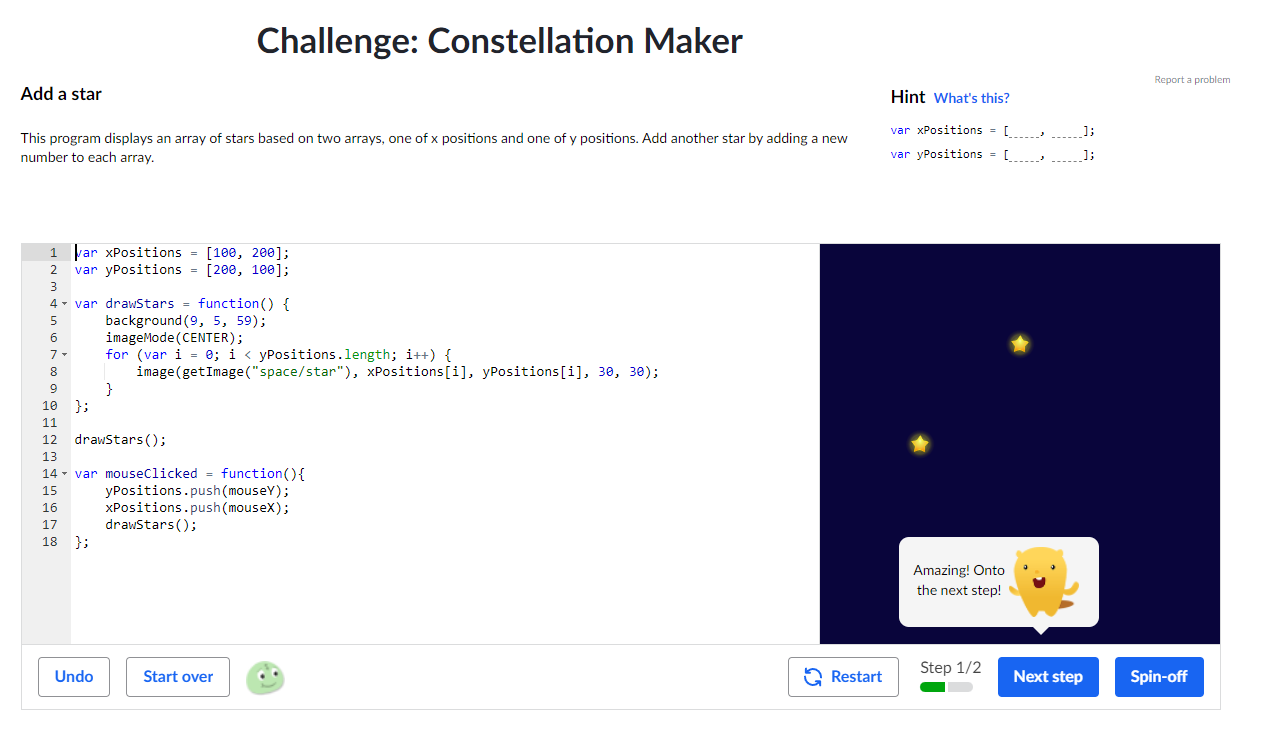
\includegraphics[width=1\linewidth]{assets/similar-games/khanacademy.png}
    \caption{Khan Academy~\cite{a2022_khan}}
    \label{fig:khanacademy}
\end{figure}

Khan Academy is one of the most extensive generic purpose educational applications with gamification elements.
\textcquote{a2022_khan}{For every student, every classroom. Real results.}
They provide interactive learning materials for math, science, history, economics, etc.
It includes instructional videos supplemented by interactive quizzes and study materials.

Focused on the programming aspects,
the application contains the Computer programming course, which covers an intro to JS, HTML, CSS, and SQL. The College Computer Science Principles course covers digital information, the Internet, cybersecurity, programming, algorithms, simulations, and data analysis.
Compared with the designed application, these courses draw on canvas in JavaScript or do websites using HTML and CSS.

It also provides a feature to create and manage classes.
Therefore, teachers can create a class and invite their students to join.
Then, teachers can create assignments and see students' performances, scores, etc.

According to~\ref{fig:khanacademy}, Khan Academy is available in more than 50 languages.
They are partnered with several schools in the United States.
And they have more than 130 million registered users in more than 190 countries.
For kids aged 2 to 8, there is also a learning game-like application called Khan Academy Kids that provides a joyful and engaging learning curriculum for young children.

\pagebreak
\begin{description}
    \item[comprehensibility] The scale of mentioned courses is relatively large, which can be confusing. Still, it also includes different types of lessons, like interactive coding videos where a code can be changed in real-time.
    \item[story] No.    
    \item[study materials] The applications provide explanation videos, text, interactive videos, etc.
    \item[graphics] Simple interface. Programming is done using a standard code editor with languages like JavaScript.
    \item[feedback] Users gain points for completing quizzes, watching learning videos, or completing other tasks. They also have badges. 
    \item[price] Free to use.
\end{description}

\newpage
\section{CodeCombat}
\label{similar-games:code-combat}

\begin{figure}
    \centering
    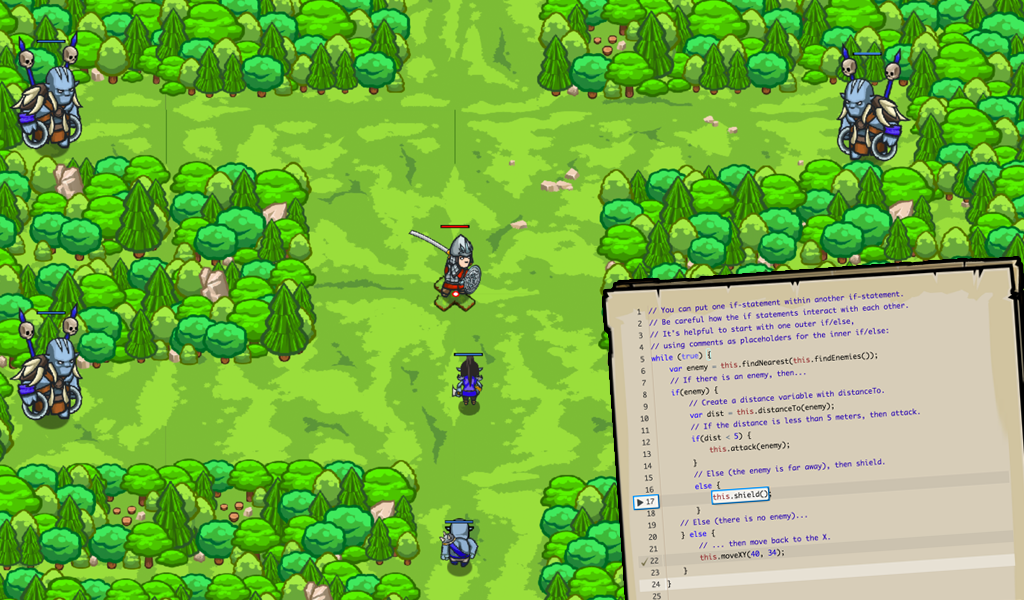
\includegraphics[width=1\linewidth]{assets/similar-games/codecombat.png}
    \caption{CodeCombat~\cite{a2022_codecombat}}
    \label{fig:codecombat}
\end{figure}

CodeCombat is a game that controls players by programming them.
It is a community project where volunteers create levels and add features.
Players have their characters with stats and items that add new features to the player in a game.

As CodeCombat mentions~\cite{a2022_codecombat}, \textquote{Programming is magic.}
They provide wizard-like features to players so they can use their pure imagination to solve game missions.
And according to the game, this approach enables players to learn faster.

\begin{description}
    \item[comprehensibility] The game clearly expresses its goals but might be overwhelming for inexperienced users.
    \item[story] Contains multiple courses with different stories.  
    \item[study materials] Does not contain a theoretical explanation for its concepts but teaches the concept by playing.
    \item[graphics] Engaging game interface that includes programming in standard programming languages like Python and JavaScript. 
    \item[feedback] Users gain points for completing game missions. These points can be used to get additional equipment.
    \item[price] Free to use for all of its core levels. Players can upgrade to a \$9.99 per month subscription, adding extra levels and in-game bonus currency.
\end{description}

\pagebreak
\section{Minecraft}
\label{similar-games:minecraft}

\begin{figure}
    \centering
    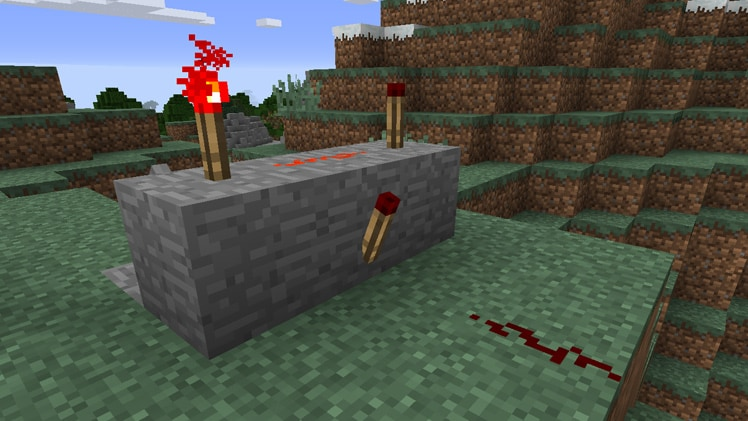
\includegraphics[width=1\linewidth]{assets/similar-games/minecraft.jpg}
    \caption{Minecraft~\cite{a2022_minecraft}}
    \label{fig:minecraft}
\end{figure}

Minecraft is the most famous building game.
Its minimalistic graphics, where all worlds are made out of cube blocs, support creative thinking and creating experiences.
It also has an Education Edition, which focuses on generic purpose education.
That means people can play or create different educational content in the Minecraft world for any subject.
Bot Minecraft Education Edition and Minecraft have ways of introducing programming to children.
Education Edition has programming courses, and Minecraft, the game itself, has programming done by players using a unique entity, a Redstone dust, and other blocs that can receive, transmit or produce a Redstone signal.

\begin{description}
    \item[comprehensibility] Both Minecraft and its Education Edition have challenging beginnings in learning to program.
    \item[story] Does not have a story dedicated to programming in the game. Courses in its Education Edition often contain stories.
    \item[study materials] Minecraft does not explain the concepts of Redstone. Its Education Edition has study materials as part of its tutorials.
    \item[graphics] Unique pixel graphics. For programming, Minecraft uses Redstone in-game mechanism.
    \item[feedback] Does not have a scoring system, but the game provides feedback.
    \item[price] Minecraft costs 23.95€, and anyone can play education Edition with a Microsoft 365 account.
\end{description}

\pagebreak
\section{Opus Magnum}
\label{similar-games:opus-magnum}

\begin{figure}
    \centering
    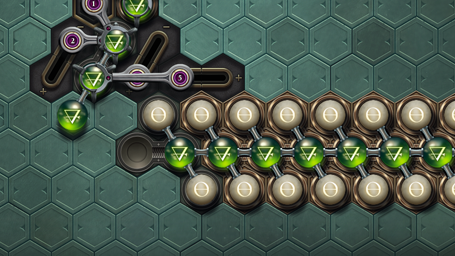
\includegraphics[width=1\linewidth]{assets/similar-games/opusmagnum.png}
    \caption{Opus Magnum~\cite{a2022_zachtronics}}
    \label{fig:opusmagnum}
\end{figure}

Opus Magnum is an alchemical game where your goal is to assemble potions, move them, transmute, etc., to complete open-ended puzzles.
Players can also compete against their friends.

The game contains a transmutation engine.
This engine allows players to place machines that operate according to a program.

Players are challenged to make their engines smaller and faster and embrace symmetry and infinity.
The game also contains a solitaire minigame.

\begin{description}
    \item[comprehensibility] The game can be a little confusing, especially for inexperienced people.
    \item[story] Contains a sophisticated story with other alchemists.
    \item[study materials] Explains basics of concepts inside of a story. 
    \item[graphics] Contains interested alchemical-inspired graphics where programming is done using the transmutation engine.
    \item[feedback] Provides a feedback of cost, cycles, and area statistics in which friends can compete.
    \item[price] 16.79€ 
\end{description}

\pagebreak
\section{7 Billion Humans}
\label{similar-games:7-billion-humans}

\begin{figure}
    \centering
    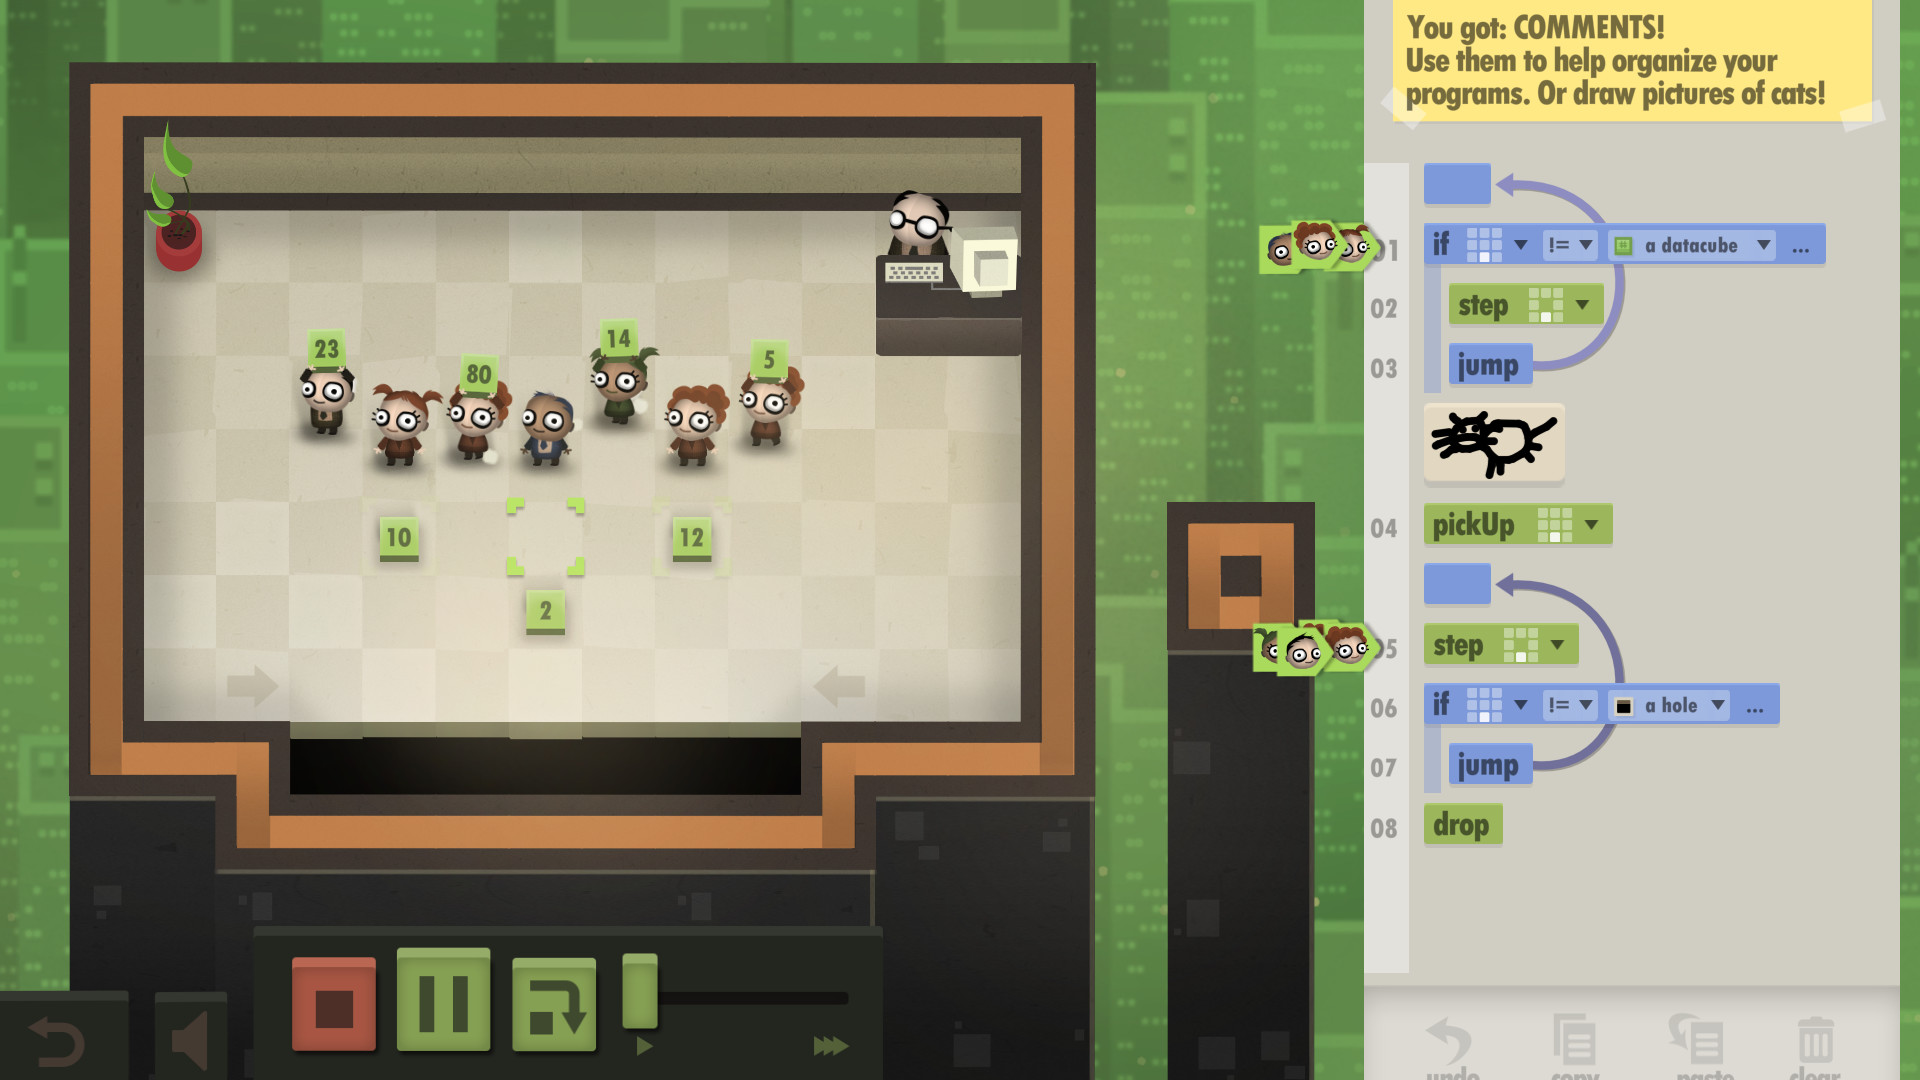
\includegraphics[width=1\linewidth]{assets/similar-games/7bilionhumans.jpg}
    \caption{7 Billion Humans~\cite{a2022_tomorrow}}
    \label{fig:7bilionhumans}
\end{figure}

7 Billion Humans is a puzzle game where your task is to program a parallel computer made of people.
Therefore, the player's job is to figure out how to synchronize workers to achieve the expected outcome.

The biggest drawback for inexperienced players might be that the game does not explain the concepts.
But the concepts are simple so that players can get into it quickly.

\begin{description}
    \item[comprehensibility] Has simple graphics, and the task is well explained.
    \item[story] Has a story in the background that is part of the game identity but is not extensive.
    \item[study materials] Does not explain the concepts in detail but provides some hints.
    \item[graphics] A simple, stylish graphics with programming with visual blocs.
    \item[feedback] Has size and speed metrics that players optionally complete for additional scores.
    \item[price] 12.49€
\end{description}

\pagebreak
\section{Evaluation}

All mentioned games are joyful and engaging.
However, none of them provide the right combination of free availability, storytelling, and study materials.
Therefore a game with gamification features mentioned in chapter~\ref{analysis} will be designed and implemented.

Every analyzed similar game has unique features from which the designed game can inspire. 
Scratch, 7~Billion Humans, and Opus Magnum have joyful visual programming tools.
CodeCombat has a great story set in gaming missions that draw players deeper.
Khan Academy has an extensive curriculum.
And Minecraft has a uniquely integrated programming feature to the in-game world.

The designed game should incorporate all these games' benefits into itself.
The game should have good storytelling, create a joyful visual programming tool that can be easily understood by children, and provide a way how players can learn basic and advanced concepts. 



\blind[25] % 4 kapitoly * 3od + víc textu u každého * 1od